\documentclass[a4paper,12pt]{article}
\usepackage[utf8]{inputenc}
\usepackage{geometry}
\usepackage{graphicx}   % images
\usepackage{fancyhdr}   % headers/footers
\usepackage{tcolorbox}
\usepackage{listings}
\usepackage{xcolor}
\usepackage{float}
\geometry{margin=1in}

% ---------- Header ----------
\setlength{\headheight}{36pt}
\setlength{\headsep}{18pt}
\renewcommand{\headrulewidth}{0.4pt}
\fancyhf{}
\fancyhead[L]{
\includegraphics[width=0.13\textwidth, keepaspectratio]{Figures/UM6Plogo.png}}
\fancyhead[R]{
\includegraphics[width=0.13\textwidth, keepaspectratio]{Figures/CC.jpg}}
\fancyfoot[L]{Data Management Lab}
\fancyfoot[R]{Prof. Karima Echihabi}
\fancyfoot[C]{Page \thepage}

% ---------- Deliverable Template ----------
\begin{document}
\thispagestyle{empty}
\begin{center}
  
\includegraphics[width=0.25\textwidth]{Figures/UM6Plogo.png}\hfill
  
\includegraphics[width=0.25\textwidth]{Figures/CC.jpg}
  \vspace{1.2cm}

  {\LARGE \textbf{Deliverable 1: Conceptual design of the Moroccan National Health Service Data Management System}}\\[0.6cm]
  {\large \textbf{Data Management Course}}\\[0.2cm]
  {\large UM6P College of Computing}\\[0.8cm]

  {\normalsize \textbf{Professor:} Karima Echihabi \quad 
   \textbf{Program:} Computer Engineering}\\[0.1cm]
  {\normalsize \textbf{Session:} Fall 2025}\\[1cm]

  \rule{0.9\textwidth}{0.5pt}\\[0.5cm]
  {\large \textbf{Team Information}} \\[0.3cm]
  \begin{tabular}{|l|l|}
    \hline
    \textbf{Team Name} & alfari9 alkhari9 \\ \hline
    \textbf{Member 1}  & Ilyas Rahmouni \\ \hline
    \textbf{Member 2}  & Malak Koulat   \\ \hline
    \textbf{Member 3}  & Aymane Raiss   \\ \hline
    \textbf{Member 4}  & Zakaria Harira   \\ \hline
    \textbf{Member 5}  & Youness Latif   \\ \hline
    \textbf{Member 6}  & Rayane Khaldi   \\ \hline
    \textbf{Member 7}  & Younes Lougnidi   \\ \hline
    \textbf{Repository Link} & \texttt{https://github.com/...} \\ \hline
  \end{tabular}
  \rule{0.9\textwidth}{0.5pt}\\
\end{center}
\clearpage
\pagestyle{fancy}

% ---------- Sections for Students ----------
\section{Introduction}

This document provides an overview of the MNHS (Moroccan National Health Services) Database Design Project. The goal of this project is to create a conceptual database model that can facilitate a national health service system's operations.

The project will focus on designing an Entity-Relationship (ER) diagram representing key entities such as patients, staff, hospitals, departments, appointments, prescriptions, medications, insurance, billing, and emergencies. The aim is to develop a database that can support real-world health service workflows such as patient management, clinical activities, prescriptions, insurance billing, and emergency care.

\section{Requirements}
\begin{enumerate}
    \item \textbf{Design an ER Diagram:} Create a complete Entity-Relationship diagram that models the entire MNHS system.
    
    \item \textbf{Model Core Entities:} The diagram must include the following entities:
    \begin{itemize}
        \item Patients
        \item Staff (with sub-types like Practitioners, Caregiving, and Technical staff)
        \item Hospitals
        \item Departments
        \item Appointments
        \item Prescriptions
        \item Medications
        \item Insurance
        \item Bills
        \item Emergencies
        \item Pharmacy Inventory
    \end{itemize}
    
    \item \textbf{Capture Specific Attributes:} Ensure each entity has the specific attributes listed in the scenario (e.g., Patient's CIN and blood group, Medication's strength and manufacturer).
    
    \item \textbf{Define Relationships:} Establish all necessary relationships between the entities, such as:
    \begin{itemize}
        \item Staff assigned to Departments.
        \item Appointments linking Patients and Staff.
        \item Prescriptions connecting Patients, Staff, and Medications.
    \end{itemize}
    
    \item \textbf{Implement Business Rules:} Model the specific constraints from the requirements, including:
    \begin{itemize}
        \item A patient can have multiple contact addresses and multiple insurance plans.
        \item A bill is linked to only one insurance and one clinical activity.
        \item A department belongs to one hospital.
    \end{itemize}
    
    \item \textbf{Write a One-Page Rationale:} Explain the key decisions made during the design process.
    
    \item \textbf{Meet the Deadline:} Submit the ER diagram and rationale by \textbf{September 24th at 23:59}.
\end{enumerate}

\section{Methodology}
\subsection{Requirement Analysis}

The first step consisted of identifying the core entities and interactions in the healthcare domain. This was achieved through reviewing existing workflows in hospitals and clinics, focusing on patients, staff, prescriptions, appointments, insurance, and billing. Functional requirements such as appointment scheduling, prescription management, and inventory tracking were clearly outlined.

\subsection{Conceptual Modeling}

An ER model was constructed to capture the relationships between the identified entities. The ER diagram illustrates the main components of the system:

\begin{itemize}
    \item \textbf{Patient information}: CIN, name, date of birth, contact details.
    \item \textbf{Medical activities}: prescriptions, medications, and appointments.
    \item \textbf{Administrative entities}: insurance, billing, and departments.
    \item \textbf{Resource management}: hospital departments, staff allocation, and pharmacy inventory.
\end{itemize}

This model allowed us to represent both clinical and administrative processes in a coherent structure.

\section{Implementation \& Results}

In this section, we present the conceptual Entity-Relationship Diagram (ER) of the MNHS database. The ER Diagram captures the main entities such as Patients, Staff, Hospitals, Departments, Appointments, Prescriptions, Medications, Insurance, Billing, and Emergencies, along with their relationships.

\begin{figure}[H]
    \centering
    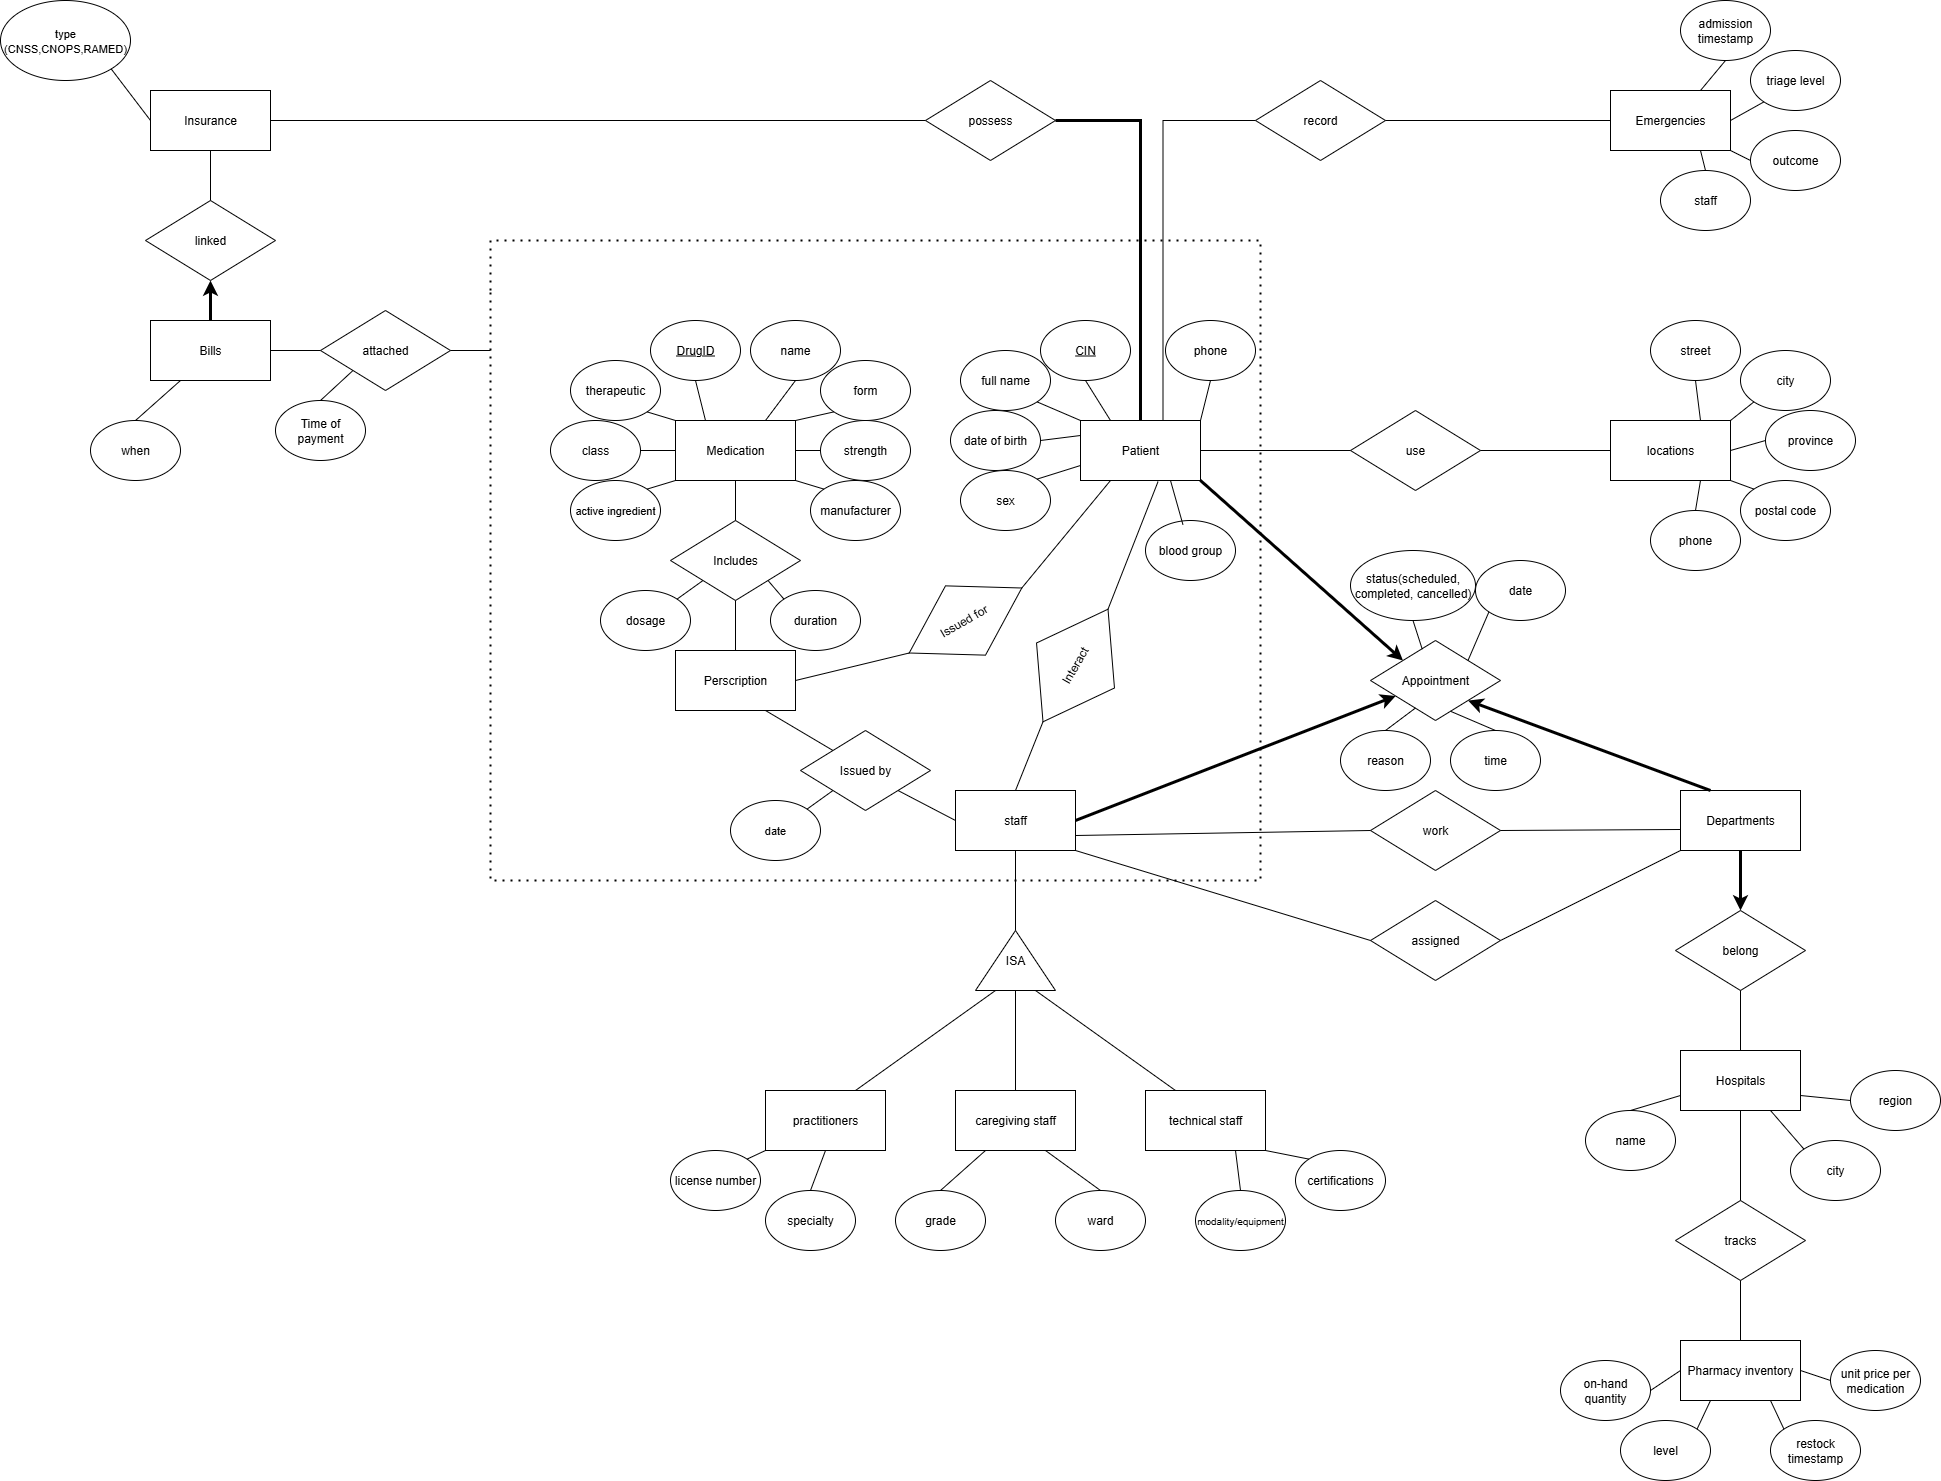
\includegraphics[width=\textwidth]{Figures/ERDFinal.png}
    \caption{Conceptual ER Diagram of the MNHS Database}
    \label{fig:erd}
\end{figure}

\section{Discussion}
While creating the ER diagram we did run into some issues. First, there were too many connections between people like patients, staff, and appointments which made the diagram to look cluttered and hard to visualize. Second, identifying the main object (an entity) or just a connection between objects (a relationship) did sometimes get confusing. Lastly the detail of choosing to show simple two-way connections or type three-way connections was not always clear.

\section{Conclusion}
This project develops a data model that was organized and coherent, reflecting the operational needs of the Moroccan National Health Services (MNHS). A data structure was created to reflect the actual interactions with patients, staff, hospitals, appointments, prescriptions, insurance, emergencies, and pharmacy inventory through an adequate analysis of the components of the system. 

The data model ensures organized and consistent data management while maintaining a model that can be extended as needed or utilized for analytical purposes. The model is also constructed in a way that establishes a clear path for implementation in a relational database system in which the conceptual schema can be represented through SQL in the form of normalized tables, defined relation constraints, and integrity constraints. 

Ultimately, this work provides an adequate starting point for an information system that could support essential functions of healthcare. Overall, this study aligns the data model with practice, supporting the reliability, scalability, and clarity that are essential in public health data management.

\end{document}
